\begin{figure}[htb!]
            \centering
            \subfigure[Linguistics]{
                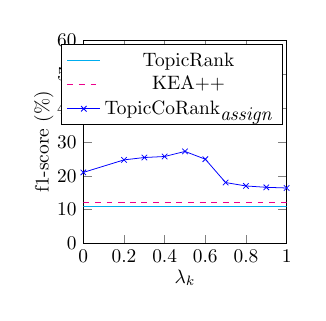
\begin{tikzpicture}[scale=.7]
                    \pgfkeys{/pgf/number format/.cd, fixed}
                    \begin{axis}[x=0.304152\linewidth,
                                 xtick={0, 0.2, 0.4, ..., 1},
                                 xmin=0,
                                 xmax=1,
                                 xlabel=$\lambda_k$,
                                 x label style={yshift=.34em},
                                 y=0.0050692\linewidth,
                                 ytick={0, 10, 20, ..., 100},
                                 ymin=0,
                                 ymax=60,
                                 ylabel=f1-score (\%),
                                 y label style={yshift=-.5em}]
                        \addplot[cyan] coordinates{
                            (0.0, 11)
                            (0.2, 11)
                            (0.3, 11)
                            (0.4, 11)
                            (0.5, 11)
                            (0.6, 11)
                            (0.7, 11)
                            (0.8, 11)
                            (0.9, 11)
                            (1.0, 11)
                        };
                        \addplot[magenta, dashed] coordinates{
                            (0.0, 12)
                            (0.2, 12)
                            (0.3, 12)
                            (0.4, 12)
                            (0.5, 12)
                            (0.6, 12)
                            (0.7, 12)
                            (0.8, 12)
                            (0.9, 12)
                            (1.0, 12)
                        };
                        \addplot[blue, mark=x] coordinates{
                            (0.0, 21.0)
                            (0.2, 24.7)
                            (0.3, 25.4)
                            (0.4, 25.7)
                            (0.5, 27.2)
                            (0.6, 24.9)
                            (0.7, 18.0)
                            (0.8, 17.0)
                            (0.9, 16.6)
                            (1.0, 16.4)
                        };
                        \legend{TopicRank, KEA++, TopicCoRank$_\textit{assign}$};
                    \end{axis}
                \end{tikzpicture}
            }
            \subfigure[Information Science]{
                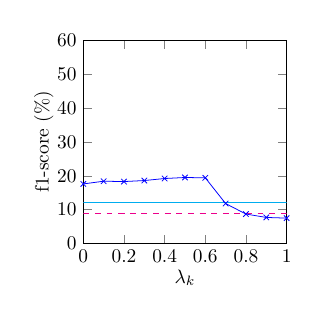
\begin{tikzpicture}[scale=.7]
                    \pgfkeys{/pgf/number format/.cd, fixed}
                    \begin{axis}[x=0.304152\linewidth,
                                 xtick={0, 0.2, 0.4, ..., 1},
                                 xmin=0,
                                 xmax=1,
                                 xlabel=$\lambda_k$,
                                 x label style={yshift=.34em},
                                 y=0.0050692\linewidth,
                                 ytick={0, 10, 20, ..., 100},
                                 ymin=0,
                                 ymax=60,
                                 ylabel=f1-score (\%),
                                 y label style={yshift=-.5em}]
                        \addplot[cyan] coordinates{
                            (0.0, 12)
                            (0.2, 12)
                            (0.3, 12)
                            (0.4, 12)
                            (0.5, 12)
                            (0.6, 12)
                            (0.7, 12)
                            (0.8, 12)
                            (0.9, 12)
                            (1.0, 12)
                        };
                        \addplot[magenta, dashed] coordinates{
                            (0.0, 9)
                            (0.2, 9)
                            (0.3, 9)
                            (0.4, 9)
                            (0.5, 9)
                            (0.6, 9)
                            (0.7, 9)
                            (0.8, 9)
                            (0.9, 9)
                            (1.0, 9)
                        };
                        \addplot[blue, mark=x] coordinates{
                            (0.0, 17.6)
                            (0.1, 18.4)
                            (0.2, 18.3)
                            (0.3, 18.6)
                            (0.4, 19.2)
                            (0.5, 19.5)
                            (0.6, 19.4)
                            (0.7, 11.8)
                            (0.8, 8.7)
                            (0.9, 7.7)
                            (1.0, 7.5)
                        };
                    \end{axis}
                \end{tikzpicture}
            }
            \subfigure[Archaeology]{
                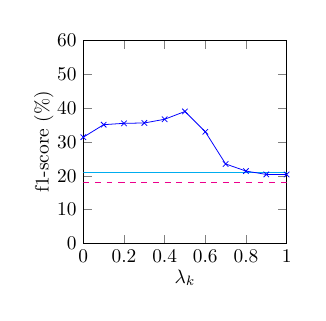
\begin{tikzpicture}[scale=.7]
                    \pgfkeys{/pgf/number format/.cd, fixed}
                    \begin{axis}[x=0.304152\linewidth,
                                 xtick={0, 0.2, 0.4, ..., 1},
                                 xmin=0,
                                 xmax=1,
                                 xlabel=$\lambda_k$,
                                 x label style={yshift=.34em},
                                 y=0.0050692\linewidth,
                                 ytick={0, 10, 20, ..., 100},
                                 ymin=0,
                                 ymax=60,
                                 ylabel=f1-score (\%),
                                 y label style={yshift=-.5em},
                                 legend style={font=\footnotesize}]
                        \addplot[cyan] coordinates{
                            (0.0, 21)
                            (0.2, 21)
                            (0.3, 21)
                            (0.4, 21)
                            (0.5, 21)
                            (0.6, 21)
                            (0.7, 21)
                            (0.8, 21)
                            (0.9, 21)
                            (1.0, 21)
                        };
                        \addplot[magenta, dashed] coordinates{
                            (0.0, 18)
                            (0.2, 18)
                            (0.3, 18)
                            (0.4, 18)
                            (0.5, 18)
                            (0.6, 18)
                            (0.7, 18)
                            (0.8, 18)
                            (0.9, 18)
                            (1.0, 18)
                        };
                        \addplot[blue, mark=x] coordinates{
                            (0.0, 31.4)
                            (0.1, 35.1)
                            (0.2, 35.5)
                            (0.3, 35.6)
                            (0.4, 36.7)
                            (0.5, 39.0)
                            (0.6, 33.0)
                            (0.7, 23.5)
                            (0.8, 21.4)
                            (0.9, 20.4)
                            (1.0, 20.4)
                        };
                    \end{axis}
                \end{tikzpicture}
            }
            \caption{
                Behavior of TopicCoRank$_\textit{assign}$ depending on $\lambda_k$ ($\lambda_t = 0.1$)
                \label{fig:lambda_k_variation}
            }
        \end{figure}